\documentclass[12pt,a4paper]{report}
\usepackage[margin=2cm]{geometry}
\usepackage{indentfirst}
\usepackage{mathrsfs}
\usepackage{amsthm}
\usepackage{CJKutf8}
\usepackage{amssymb}
\usepackage{amsmath}
\usepackage{import}
\usepackage{xifthen}
\usepackage{pdfpages}
\usepackage{transparent}
\usepackage{overpic}
\usepackage{setspace}
\usepackage{rotating}
\usepackage{graphicx}
\usepackage{wasysym}
\usepackage{xcolor}
\usepackage{biblatex}
\addbibresource{reference.bib}
\usepackage{mathtools}
\theoremstyle{definition} 
\newtheorem*{remark}{Remark} 

\usepackage{newtxmath} % For chalk font 1. \vmathbb{1}

\pagestyle{empty}
\newcommand{\iso}{\mathrm{iso}}
\newcommand{\esc}{\mathrm{esc}}
\newcommand{\oversim}[1]{\parbox[t][-18pt][c]{10pt}{\scriptsize$\sim$}\hspace*{-12pt}{#1}}
\newcommand{\bbar}[1]{\overline{#1}}
\newcommand{\ul}[1]{\underline{#1}}
\newcommand{\SOL}{\fbox{ \tt s\parbox[b][2pt][c]{6pt}{o}\hspace*{-7pt} L:}}
\newcommand{\sixedge}{\mbox{\parbox[t][-2pt][c]{10pt}{\scriptsize$\blacktriangledown\hspace{-3.6pt}\blacktriangle\hspace{-4pt}\blacktriangledown$}\hspace{-10.2pt}\parbox[b][10.7pt][c]{10pt}{\scriptsize$\blacktriangle\hspace{-3.6pt}\blacktriangledown\hspace{-3.6pt}\blacktriangle$}}}
\newcommand{\indecate}{\mbox{\begin{turn}{65.9}
$>$
\end{turn}\hspace{-10.5pt}\parbox[t][-5pt][c]{10pt}{$\bot$}\hspace{-4.35pt}\parbox[t][-3.4pt][c]{4pt}{$\shortmid$}}}
\newcommand{\incfig}[1]{%
\import{./picture/}{#1.pdf_tex}
}

\begin{document}
\section*{Russo-Seymour-Welsh Theory}

In this section, we discuss the scale invariant property of some connecting events when $p=p_c$ on $\mathbb{Z}^2$ lattice. In particular, we presents the invariant behaviour of the \textit{horizontal crossing event in a rectangle of size $[0,\rho n]\times[0,n]$}, which is denoted by $\mathcal{H}(\rho n, n)$.\\ \\
\textbf{Theorem (Russo-Seymour-Welsh).}
\textit{Let $\rho>0$. There exists $c=c(\rho)>0$ such that for all $n\geq 1$, we have}
\begin{equation*}
c\leq\mathbb{P}_{\frac{1}{2}}\big[\mathcal{H}(\rho n, n)\big]\leq 1-c,
\end{equation*}
\textit{where $\mathcal{H}(\rho n, n)$ denotes the horizontal crossing event in a rectangle with size $[0,\rho n]\times [0,n]$.}\\ \\
They proved this theorem by proving a special case:\\
\textbf{Theorem.} \textit{For all }$n\geq 1$,
\begin{equation*}
\mathbb{P}_{\frac{1}{2}}\big[\mathcal{H}(3n,2n)\big]\geq\frac{1}{128}.
\end{equation*}\\
Once one get this result, i.e. when one find $c(\rho)$ for some $\rho>1$ (e.g. $c(3/2)$), then one can get $c(\rho')$ for arbitrary $\rho'>1$ by construct the crossing events $\mathcal{H}(\rho n,n)$ that assures $\mathcal{H}(\rho'n, n)$ to occur, and hence we can prove the first theorem. For example, to get a lower bound for $\mathbb{P}_{p_c}[\mathcal{H}(4n,n)]$, we can place five $(2n,n)$ boxes as follows: Let $R_1=[0,2n]\times[0,n]$, $R_2=[n,2n]\times[-n,n]$, $R_3=[n,3n]\times[-n,0]$, $R_4=[2n,3n]\times[-n,n]$ and $R_5=[2n,4n]\times[0,n]$. Then we have
\begin{equation*}
\mathbb{P}_{p_c}[\mathcal{H}(R_1)\cap\mathcal{V}(R_2)\cap\mathcal{H}(R_3)\cap\mathcal{V}(R_4)\cap\mathcal{H}(R_5)]\leq\mathbb{P}_{p_c}[\mathcal{H}([0,4n]\times[0,n])].
\end{equation*}
Now by Harris-FKG inequality and translation invariant property on $\mathbb{Z}^2$ lattice, we immediately have
\begin{equation*}
c(2)^5\leq \mathbb{P}_{p_c}[\mathcal{H}(4n,n)].
\end{equation*}

With Russo-Seymour-Welsh's theory, we're able to give a scale invariant property for more general crossing events. Consider a simply connected domain with a smooth boundary $\Omega$ with distinct boundary points $a,b,c,d$. For $\delta>0$, we define a finite graph $\Omega^\delta=\delta\mathbb{Z}^2\cap\Omega$. And let $a^\delta, b^\delta, c^\delta, d^\delta\in\Omega^\delta$ to be the closest points to $a,b,c,d\in\partial\Omega$. Also define $(a^\delta b^\delta),\,(c^\delta d^\delta)$ as the paths on $\partial\Omega^\delta$ from $a^\delta$ to $b^\delta$, from $c^\delta$ to $d^\delta$ counterclockwise.\\ \\
\textbf{Theorem.} \textit{
There exists $c=c(\Omega,a,b,c,d)>0$ such that for any $\delta>0$,}
    \begin{equation*}
        \mathbb{P}_\frac{1}{2}\big[(a^\delta b^\delta)\xleftrightarrow{\text{$\Omega^\delta$}}(c^\delta d^\delta)\big]\geq c.
    \end{equation*}
    
    \begin{figure}[b]
    		\centering
        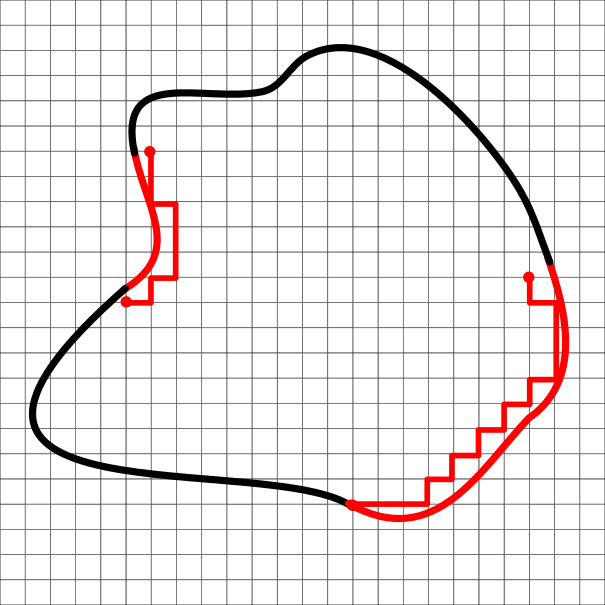
\includegraphics[width=5.0cm]{omega_2.png}
       	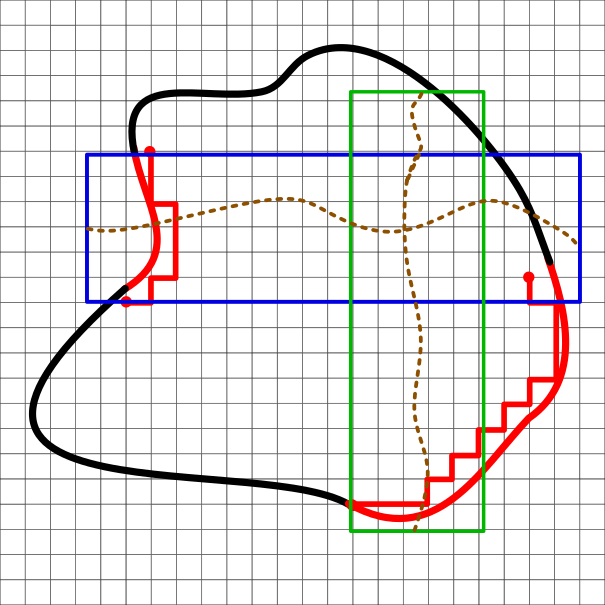
\includegraphics[width=5.0cm]{omega_2_crossing.png}
    \end{figure}

\end{document}